%!TEX root = /Users/stwaidele/Dropbox (Leisinger)/02 - AKAD/Projektbericht/Möglichkeiten der Digitalen Kontaktaufnahme im Endkundenbereich/vorlage.tex

\section{Einsatzorte} % (fold)
\label{sec:einsatzorte}

\subsection{Quellmedien} % (fold)
\label{sub:quellmedien}
Rein technisch betrachtet ist das Quellmedium beim Untersuchten Meidenbruch bin zur digitalen Kommunikation meist ein Druckerzeugnis. Dies kann der Briefbogen, das Hausprospekt, eine Broschüre, ein Schild, Plakat oder die Visitenkarte sein. Das Wechselmedium ist entweder direkt darauf gedruckt, oder im Falle von elektronischen Varianten hinter einem entsprechenden Logo oder Hinweistext platziert. Möglich wären zwar auch Werbespots. In der klassischen Form des Werbespots sind diese für die betrachtete  Unternehmensgröße jedoch zu teuer.

% subsection quellmedien (end)

\subsection{An Stationen des Customer Journey} % (fold)
\label{sub:stationen_des_customer_journey}
Es sind diejenigen Phasen der Customer Journey bei denen der Gast direkten Kontakt hat, während denen gastronomische Betriebe die digitale Kontaktaufnahme beeinflussen können. Dies beginnt bei der Buchung, ist in der Erlebnisphase am ausgeprägtesten und reicht bis zur Nachbereitung.

Während des Aufenthalts können entsprechende Hinweise auf Drucksachen und Schildern platziert werden um den Gast auf die digitalen Angebote des Betriebs zu führen. Dies kann an jedem \ac{POI}, also an Sehenswürdigkeiten jeglicher Art wie zum Beispiel an einem Gemälde, am Speisekartenaushang, an der Eingangstür oder im Rosengarten sein.

Bei Buchung und Nachbereitung sind diese Hinweise in der Korrespondenz zu platzieren.\footnote{Im Falle von E–Mails wird somit ein Wechsel von persönlicher zu unpersönilicher elektronischer Kommunikation angestrebt.}
% subsection stationen_des_customer_journey (end)

\subsection{In der Gastronomie} % (fold)
\label{sub:gastronomie}
In gastronomischen Betrieben lässt sich der Aufenthalt bzw. die Erlebnisphase der Customer Journey vereinfacht in fünf Phasen einteilen: Vor dem Besuch, vor der Bestellung, nach der Bestellung, während des Verzehrs\footnote{Bei mehrgängigen Menüs durch wartezeiten auf den nächsten Gang unterbrochen} und nach dem Besuch. Die Phasen eignen sich unterschiedlich gut für die digitale Kontaktaufnahme.  Vor der Bestellung und während des Verzehrs sind Verzögerungen durch den Gebrauch von Smartphones nicht wünschenswert.\footnote{Auch wenn die Behauptungen, dass der Service in einem New Yorker Restaurant sich durch Smartphonenutzung um durchschnittlich 50 Minuten verzögert wird (vgl. \cite{craiglist:slow}) nicht belegt sind, sind die geschilderten Phänomene zumindest mit kürzeren Zeitangaben doch plausibel. (vgl. \cite{craiglist:fake})} Vor dem Besuch, nach der Bestellung sowie nach den Besuch entstehen hierdurch keine Probleme, sondern für Gast und Betrieb vorteilhafte Anwendungsfälle. 

Der Gast kann durch entsprechende Hinweise am Speisekartenaushang, im Eingangsbereich, auf der Speisekarte, auf Tischaufstellern oder auf der Rechnung zu den digitalen Angeboten des Betriebs geleitet werden.
% subsection gastronomie (end)

\subsection{In der Hotellerie} % (fold)
\label{sub:hotellerie}
In Beherbergungsbetrieben hält sich der Gast während des Aufenthalts zwischen Anreise (Check–In) und Abreise (Check–Out) an unterschiedlichen Orten innerhalb des Betriebs auf. Für die Einnahme der Mahlzeiten gilt das im Abschnit~\myref{sub:gastronomie} gesagte. Weitere mögliche Orte der digitalen Kontktaufnahme sind das Zimmer des Gastes, öffentliche Bereiche wie Flure, Aufenthaltsräume und der Wellnessbereich. Des weiteren können solche Angebote besonders an Orten, an denen viele Gäste warten, gerne angenommen werden. Beispiele hierfür sind im Bereich der Aufzüge oder in der Lobby.

% subsection hotellerie (end)


% section einsatzorte (end)

\newpage
\section{Einsatzzwecke} % (fold)
\label{sec:einsatzzwecke}

\subsection{Zielmedien} % (fold)
\label{sub:zielmedien}
Die Zielmedien können technisch in direkt und indirekt erreichte Ziele unterteilt werden. Bei direkter Zielerreichung wird die vom Gast erwartete Information direkt durch das Wechselmedium übertragen. Hierbei ist die Größe der Information durch die Speicherkapazität der verwendeten technischen Lösung begrenzt. Diese Methode funktioniert ohne Internetzugriff.  Im Gegensatz dazu wird bei der indirekten Zielerreichung lediglich eine \ac{URL} zur Information übergeben. Hierbei ist die Datenmenge lediglich durch die Bandbreite bzw. durch die Geduld des Kundens begrenzt.
% subsection zielmedien (end)

\subsection{Beeinflussung Customer Journey} % (fold)
\label{sub:beeinflussung_customer_journey}
Touristische Betriebe können durch Lenkung der digitalen Aktivitäten der Kunden auf Customer Journey weiterer Interessenten einwirken. Wenn zufriedene Gäste ihre Erlebnisse und Bewertungen anderen mitteilen, dann hat dies positive Auswirkungen auf deren Phasen der Inspiration, Recherche und Planung. Somit bieten sich generelle Hinweise auf Social Media Dienste an, um das Teilen der Urlaubserlebnisse zu fördern. 

\begin{figure}[H]
\begin{center}
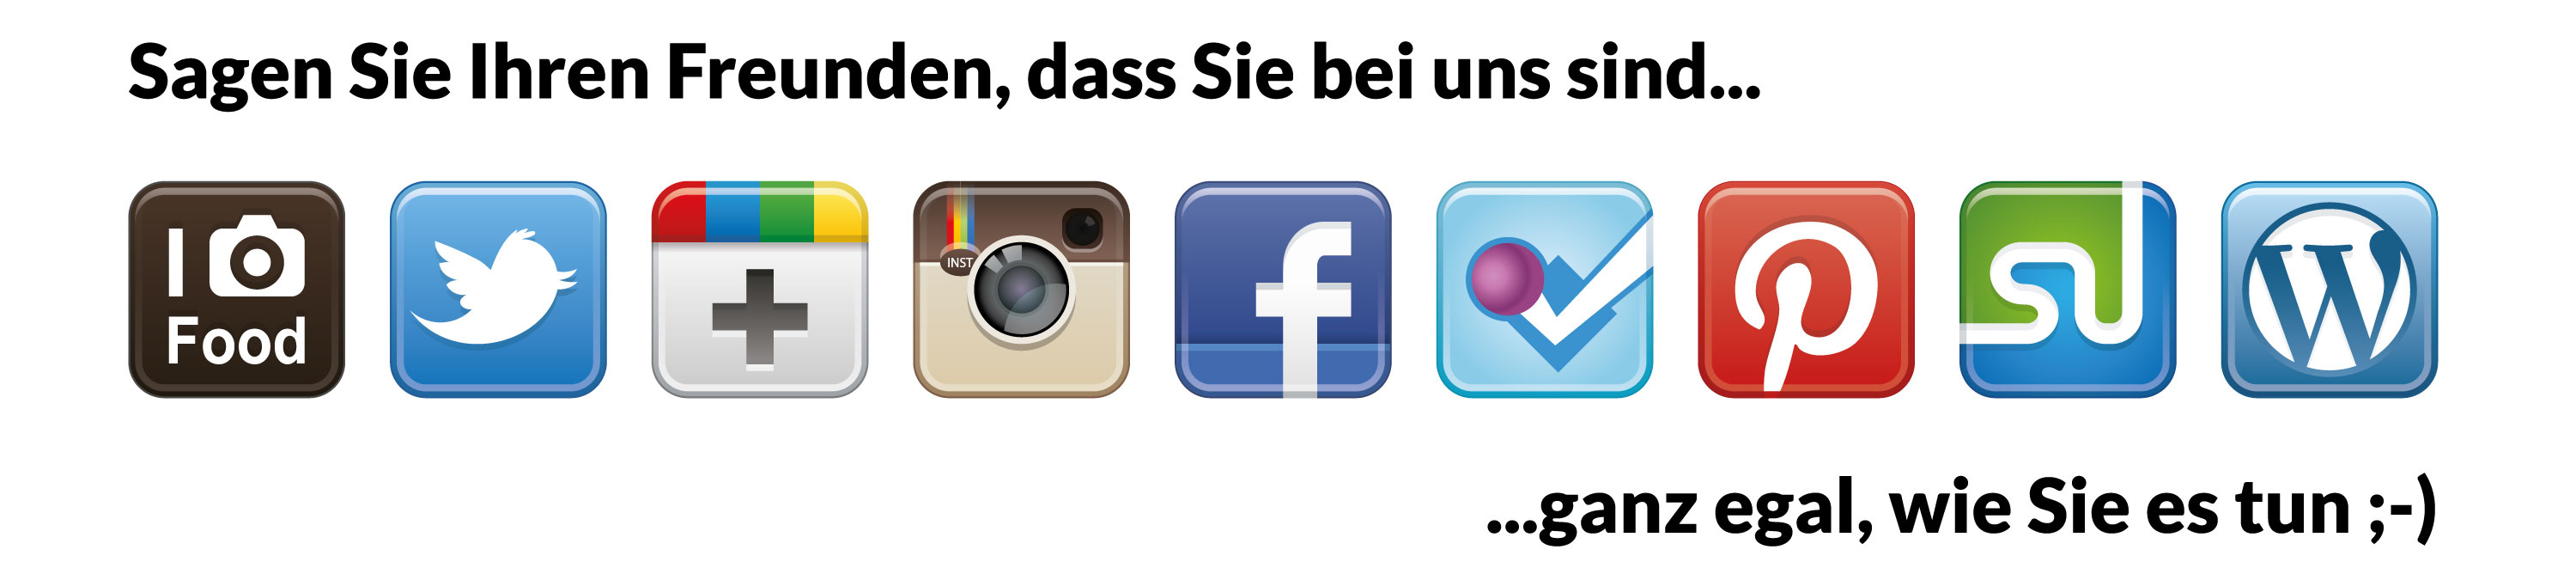
\includegraphics[width=.8\textwidth]{zielcj.jpg}
\caption[Beispiel: Hinweis auf Social Media Dienste]{Beispiel: Hinweis auf Social Media Dienste\protect\footnotemark}
\label{pic:zielcj}
\end{center}
\end{figure}
\footnotetext{Rückseite der Visitenkarte eines Hotels}

Des weiteren können Gäste gezielt auf Webseiten oder Social Media Angebote des Betriebs gelenkt werden. Hier kann der Kunde dann mit Informationen versorgt werden. Wenn der Kunde dazu animiert werden kann, die digitalen Angebote des Betriebs selbst in den Netzwerken zu teilen, werden dadurch diese im Einfluss gestärkt.\footnote{vgl. \cite{fb:news}}
% subsection beeinflussung_customer_journey (end)

\subsection{Kunden mit Information versorgen} % (fold)
\label{sub:kunde_mit_information_versorgen}
Bei ausreichender Speicherkapazität des Wechselmediums kann der Kunde direkt mit Informationen versorgt werden. Hierfür bieten sich Kontaktinformationen\footnote{Als VCard formatierte Informationen lassen sich direkt in das Adressbuch von Smartphones importieren.}, Terminkalendereinträge oder erklärende Texte\footnote{z.B. zu Bildern, oder Öffnungszeiten} an.

Während reine Informationstexte keinen oder nur sehr geringen Mehrwert gegenüber den gedruckten Informationen bieten, sind entsprechend formatierte Kontakt– oder Termininformationen für Kunden und Unternehmen nützlich, da durch sie die manuelle Eingabe in das Smartphone vermieden werden kann und somit diese Informationen wahrscheinlicher beim Kunden gespeichert werden.

Bei indirekten Zielen kann der Kunde auf Webseiten beliebiger Art geführt werden. Das Wechselmedium übergibt dazu die entsprechende \ac{URL}, die mit dem Webbrowser des Smartphones aufgerufen werden kann. Hierbei sollte es sich um eine für Mobilgeräte optimierte Seite handeln.

Mögliche Zielseiten können die Unternehmenswebsite, der Firmeneintrag bei Bewertungsdiensten, das Profil des Betriebs bei Social Media Diensten, Gewinnspiele, eine Eintragung für den Newsletter oder auch die Downloadadresse der Betriebseigenen App sein. Somit können die entsprechenden Angebote beworben bzw. entsprechende Aktivitäten gefördert werden.

% subsection kunde_mit_information_versorgen (end)

\subsection{Informationen von Kunden erhalten} % (fold)
\label{sub:informationen_vom_kunden_erhalten}
Durch den Einsatz von aktiven Elementen bzw. indirekten Zielen kann auch das Unternehmen Daten über seine Kunden sammeln. Dies kann in anonymer Form über die Zugriffsdaten der referenzierten Webseiten oder falls dies die eingesetzte Technologie dies ermöglicht einen Zugriffszähler im Wechselmedium\footnote{z.B. in Bluetooth Low Energy Geräten}. Durch mehrere Elemente kann auch der Pfad von Kunden erfasst oder geschätzt werden. Über die HTML5 Geolocation \ac{API} ließe sich sogar die exakte Position des Kunden beim Seitenabruf ermitteln.\footnote{z.B. \url{http://www.torbenleuschner.de/files/geo.htm}}

Durch entsprechende Gestaltung der referenzierten Webseite können auch personalisierte Daten erfasst werden. Hierzu ist z.B. ein Newsletterangebot, die Abfrage von Kundenfeedback oder ein Gewinnspiel geeignet. Hierbei sind jedoch unbedingt die Vorschriften des Datenschutzgesetzes zu beachten.
% subsection informationen_vom_kunden_erhalten (end)

% section einsatzzwecke (end)

\newpage
\section{Bewertung der Technologien} % (fold)
\label{sec:bewertung}

\subsection{Bewertung QR Codes} % (fold)
\label{sub:bewertung_qr_codes}
QR Codes können für alle Quellmedien und für alle Zielmedien eingesetzt werden. Der zur Erstellung von Drucksachen ohnehin notwendige Workflow wird lediglich um die Erstellung des Codes erweitert, was mit Hilfe von kostenlosen Webdiensten ohne großen Aufwand möglich ist.\footnote{z.B. \url{http://www.racoindustries.com/barcodegenerator/2d/qr-code.aspx}} Die Kosten für identische QR–Codes beschränken sich somit lediglich auf ebendiese Erstellung und bleiben unabhängig von der Ausbringungsmenge konstant. Es entstehen keine Variablen Kosten. Im Betrieb treten keine laufenden Kosten auf.

QR Codes sind mit allen gängigen Smartphones und Tablet–PCs lesbar, allerdings i.d.R. nicht mit vorinstallierter Software. Der Kunde muss somit einmalig vor der ersten Nutzung eine entsprechende Lese–App herunterladen und installieren. Vor jedem Lesen, muss diese aktiviert werden und mit der Kamera der QR Code erfasst werden. Hierbei kann es je nach Größe des gedruckten Codes, der Informationsdichte und den Lichtverhältnissen zu Fokusproblemen kommen, die das Lesen erschweren.   

Die maximale Speicherkapazität ist somit nur theoretisch erreichbar. Je größer die zu speichernde Datenmenge, desto feiner werden bei gleich bleibender Abbildungsgröße die zu scannenden Strukturen. Die Abbildungsgröße ist jedoch aufgrund der Nutzung der Smartphone–Kamera limitiert.\footnote{Auch bei extrem groß dargestellten QR–Codes muss dieser durch Anpassung des Abstandes dieser so verkleinert werden, dass er ganz von der Kamera erfasst wird.} So war keines der getesteten Smartphones\footnote{Apple iPhone 5 sowie Samsung Galaxy S5 mini} in der Lage, einen V40 QR–Code zu erkennen. Auch bei kleineren Datenmengen treten bereits deutliche Unterschiede in der Erkennungsleistung sowohl zwischen den Geräten als auch zwischen den verwendeten Apps auf. Für die Übertragung einer \ac{URL}, Kontaktinformationen oder kurze erklärende Texte ist jedoch zuverlässig möglich.

Von den 174 Teilnehmenden der Umfrage gaben lediglich 26 an, QR Codes nicht zu kennen und weitere 28, sich nicht für QR Codes zu interessieren. Der Bekanntheitsgrad von QR Codes liegt somit bei knapp 60\% (120 Personen). Von den 119 gegebenen Angaben zur Benutzerfreundlichkeit waren 93 bzw. 78\% im Bereich „Gut“ oder besser.

Von den 112 Teilnehmenden, die QR Codes nutzen, nutzen 30 (27\%) NFC Tags, 99 (88\%) Bluetooth, 12 (11\%) \ac{BLE} und 80 (71\%) Kurzlinks. Von diesen Personen bewerteten die  Benutzerfreundlichkeit von NFC Tags 22 (20\%), von Bluetooth 72 (64\%), von \ac{BLE} 4 (4\%), und von Kurzlinks 65 (58\%) im Vergleich zu QR Codes als „gleich oder besser“.

Beim Einsatz von QR Codes besteht die Möglichkeit Spoofings durch unbemerktes Überkleben mit Codes, die falsche Informationen beinhalten oder dazu führen. Diese Vorgehensweise ist besonders bei einzeln platzierten QR Codes möglich. 
% subsection bewertung_qr_codes (end)

\subsection{Bewertung NFC Tags} % (fold)
\label{sub:bewertung_nfc_tags}
NFC Tags können mit Einschränkungen für alle Quellmedien und für alle Zielmedien eingesetzt werden. Der mit einem NFC-fähigen Smartphone oder Tablet–PC beschriebene NFC Tag ist das Kontaktmedium oder wird hinter dem Medium angebracht. Durch den Preis von einigen Cent pro NFC–Aufkleber\footnote{Januar 2015: 0,35€ pro Aufkleber bei NFC-Tag-Shop.de} sowie der Notwendigkeit jeden NFC Tag einzelnen zu beschreiben entstehen bei der Ausbringung identischer Kopien auf Massenartikeln jedoch variable Kosten. Hierdurch werden die möglichen Quellmedien durch die Wirtschaftlichkeit begrenzt. Im Betrieb treten keine laufenden Kosten auf.

Es ist nicht möglich, NFC Tags mit Apple Smartphones oder Tablet–PCs zu lesen. In der aktuellen Modellgeneration ist zwar ein NFC Lesechip eingebaut. Dieser ist jedoch nicht allgemein einsetzbar, sondern der Apple–eigenen Bezahlsoftware vorbehalten.\footnote{vgl. cite{zdnet:applenfc}}
Somit sind mindestens 12,7\% der neu verkauften Smartphones nicht in der Lage, Informationen aus NFC Tags auszulesen.\footnote{\cite{garnter:os}, Tabelle 2}

Von den 174 Teilnehmenden der Umfrage gaben 72 an, NFC Tags nicht zu kennen und weitere 38, sich nicht für NFC Tags zu interessieren. Der Bekanntheitsgrad von NFC Tags liegt somit bei knapp 37\% (64 Personen). Von den 45 gegebenen Angaben zur Benutzerfreundlichkeit waren 28 bzw. 62\% im Bereich „Gut“ oder besser. 

Von den 32 Teilnehmenden, die NFC Tags nutzen, nutzen 30 (94\%) QR Codes, 30 (94\%) Bluetooth, 8 (25\%) \ac{BLE} und 26 (81\%) Kurzlinks. Von diesen Personen bewerteten die  Benutzerfreundlichkeit von QR Codes 19 (59\%), von Bluetooth 23 (72\%), von \ac{BLE} 3 (9\%), und von Kurzlinks 19 (59\%) im Vergleich zu NFC Tags als „gleich oder besser“.

Um Missbrauch zu verhindern, können NFC Tags beim Beschreiben mit einem Schreibschutz versehen werden. Dieser schließt dann aber auch spätere gewollte Änderungen an den gespeicherten Daten aus, so dass zur Aktualisierung ein neuer NFC Tag verwendet werden muss. Spoofing ist somit lediglich durch das Anbringen von weiteren NFC Tags möglich.
% subsection bewertung_nfc_tags (end)

\subsection{Bewertung Bluetooth} % (fold)
\label{sub:bewertung_bluetooth}
Um Bluetooth als Kontaktmedium zu nutzen, wird eine Sendestation benötigt, die mit dem Gerät des Kunden\footnote{Neben einem Smartphone kommen hier auch Tablet–PCs oder Notebooks mit Bluetooth–Schnittstelle in Frage} Kontakt aufnimmt und die gewünschten Daten überträgt. Die Hardwareanforderungen hierzu sind niedrig, so dass ein entsprechend programmiertes Smartphone oder ein Einplatinencomputer\footnote{z.B. Raspberry Pi oder Arduino} ausreicht. Die Sendestation kann aufgrund der Reichweite auch in einigen Metern Entfernung zur Position des Kunden platziert werden. Aufgrund dieser notwendigen Infrastruktur ist Bluetooth nicht für die Ausbringung auf Massenartikeln geeignet. Die einmaligen Kosten belaufen sich auf den Programmieraufwand für die gewünschte Funktionalität. Pro Sendestation entstehen zusätzlich variable Kosten, die von der eingesetzten Hardware abhängig sind.\footnote{z.Zt. kostet ein Raspberry Pi ca. 40€ bei \url{Amazon.de}} Während des Betriebs fallen Stromkosten an.

Alle gängigen Smartphones, Tablet–PCs und viele Notebooks können über Bluetooth mit der Sendestation Daten austauschen. Hierzu ist allerdings ein Kopplungsvorgang notwendig, der einige Sekunden dauert und die aktive Mitwirkung des Kundens erfordert\footnote{Bluetooth ggf. aktivieren, Umgebung nach Geräten durchsuchen, Verbindung bestätigen.} Anschließend ist jedoch die Übertragung von Daten entsprechend der von beiden Geräten unterstützten Protokolle möglich. Die Schnittmenge der von Sender und Empfänger unterstützen Übertragungsprotokolle beschränkt die möglichen Kontaktmöglichkeiten. So unterstützen Apple–Geräte weder die Übertragung von Texten und Bildern noch von Kontaktinformationen. Bei anderen Herstellern kann die entsprechende Unterstützung dieser Funktionalität von Gerät und Betriebssystemversion abhängig sein.

Von den 174 Teilnehmenden der Umfrage gaben 7 an Bluetooth nicht zu kennen und weitere 22, sich nicht für Bluetooth zu interessieren. Der Bekanntheitsgrad von Bluetooth liegt somit bei über 83\%. Von den 151 gegebenen Angaben zur Benutzerfreundlichkeit waren 120 bzw. 79\% im Bereich „Gut“ oder besser.

Von den 140 Teilnehmenden, die Bluetooth nutzen, nutzen 99 (71\%) QR Codes, 30 (21\%) NFC Tags, 13 (9\%) \ac{BLE} und 95 (68\%) Kurzlinks. Von diesen Personen bewerteten die  Benutzerfreundlichkeit von QR Codes 64 (46\%), von NFC Tags 22 (16\%), von \ac{BLE} 2 (1\%), und von Kurzlinks 73 (52\%) im Vergleich zu Bluetooth als „gleich oder besser“.

Missbrauch ist wegen der Reichweite von Bluetooth durch von Angreifern platzierten Sendern auch aus einigen Metern Entfernung möglich, aufgrund der benötigen Stromversorgung jedoch aufwändig. Mögliche temporäre und mobile Spoofing–Angriffe mit Smartphones, die sich als betriebseigene Sender ausgeben sind möglich und nur schwer zu bemerken. 

% subsection bewertung_bluetooth (end)

\subsection{Bewertung Bluetooth Low Energie} % (fold)
\label{sub:bewertung_bluetooth_low_energie}
Für den Einsatz von \ac{BLE} Sendern zur Kontaktaufnahme gilt aufgrund der gemeinsamen Basistechnologie zunächst das für Bluetooth gesagte. Die Sender sind jedoch fertig konfiguriert im Handel erhältlich, was die Notwendigkeit der Kopplung mit dem Empfänger. \ac{BLE} benötigt auf Kundenseite ein Bluetooth 4.0 fähiges Endgerät, welche aber bereits seit 2011 im Handel sind und eine große Menge der aktuellen und vorhergehenden Generation von Smartphones einschließt.\footnote{\cite{gilchrist}, Abschnitt 1.4}

Bei den vom Sender übertragenen Daten handelt es sich lediglich um eine weltweit eindeutige Identifikation, sowie der Entfernung zwischen Sender und Empfänger. Eine Übersetzung in für den Kunden nützliche Daten erfolgt dann in einer betriebsspezifischen Smartphone–App\footnote{Die Nutzung von betriebsspezifischen Apps wird in dieser Arbeit nicht untersucht.} oder in Form von Passbook Codes.\footnote{Dies stellt einen Spezialfall der Weitergabe von Informationen an Kunden dar.} Die Kosten pro BLE Sender betragen je nach Hersteller zwischen 8€ und 40€. Passbook Codes können zu geringen Kosten bei Internetdiensten erstellt werden.\footnote{z.B. \url{http://www.passcreator.de/preise/}} Aufgrund der technischen Voraussetzungen ist \ac{BLE} nicht für die mehrfache Ausbringung identischer Exemplare, sondern nur für an einen bestimmten Ort gebundene Quellmedien geeignet. 

Von den 174 Teilnehmenden der Umfrage gaben 117 an \ac{BLE} nicht zu kennen und weitere 28, sich nicht für \ac{BLE} zu interessieren. Der Bekanntheitsgrad von \ac{BLE} liegt somit bei 17\%. Von den 15 gegebenen Angaben zur Benutzerfreundlichkeit waren 6 bzw. 40\% im Bereich „Gut“ oder besser.

Von den 13 Teilnehmenden, die \ac{BLE} nutzen, nutzen 12 (92\%) QR Codes, 8 (62\%) NFC Tags, 13 (100\%) Bluetooth und 12 (92\%) Kurzlinks. Von diesen Personen bewerteten die  Benutzerfreundlichkeit von QR Codes 7 (54\%), von NFC Tags 6 (46\%), von Bluetooth 8 (62\%), und von Kurzlinks 8 (62\%) im Vergleich zu \ac{BLE} als „gleich oder besser“.

Missbrauch ist wie auch bei Bluetooth durch vom Angreifer platzierte Sender möglich, aufgrund der Unabhängigkeit von externen Stromquellen sogar noch einfacher. Gleiches gilt für temporäre bzw. mobile Angriffe. Neben dem Spoofing ist jedoch auch das Hacking bei BLE Sendern möglich.\footnote{vgl. \cite{gilchrist}, Abschnitt 9.2} 
% subsection bewertung_bluetooth_low_energie (end)

\subsection{Bewertung Kurzlinks} % (fold)
\label{sub:bewertung_kurzlinks}
Kurzlinks können für alle Quellmedien und mit für alle Zielmedien eingesetzt werden. Der zur Erstellung von Drucksachen ohnehin notwendige Workflow wird lediglich um die Erstellung des Links erweitert, was in \ac{CMS} ohne großen Aufwand möglich ist. Die Kosten beschränken sich somit lediglich auf ebendiese Erstellung bleiben unabhängig von der Ausbringungsmenge konstant. Es entstehen keine Variablen Kosten. Im Betrieb treten keine laufenden Kosten auf.

Kurzlinks werden vom Kunden in die Adresszeile des Webbrowsers des Smartphone, Tablet–PC oder Notebook eingegeben. Somit sind sie mit allen Geräten mit vorinstallierter Software nutzbar. 

Von den 174 Teilnehmenden der Umfrage gaben 35 an, Kurzlinks nicht zu kennen und weitere 28, sich nicht für Kurzlinks zu interessieren. Der Bekanntheitsgrad von Kurzlinks liegt somit bei über 63\%. Von den 114 gegebenen Angaben zur Benutzerfreundlichkeit waren 98 bzw. 86\% im Bereich „Gut“ oder besser. 

Von den 104 Teilnehmenden, die Kurzlinks nutzen, nutzen 80 (77\%) QR Codes, 26 (25\%) NFC Tags, 95 (91\%) Bluetooth und 12 (12\%) \ac{BLE}. Von diesen Personen bewerteten die  Benutzerfreundlichkeit von QR Codes 44 (42\%), von NFC Tags 15 (14\%), von Bluetooth 69 (66\%), und von \ac{BLE} 98 (94\%) im Vergleich zu Kurzlinks als „gleich oder besser“.

Beim Einsatz von Kurzlinks besteht die Möglichkeit des Spoofings durch unbemerktes Überkleben mit \ac{URL}s, die zu falschen Informationen führen. Des weiteren besteht die Möglichkeit, ähnliche Domainnamen, sogenannte „Tippfehler Domains“, zu registriern um die Kunden auf die Webseiten des Angreifers zu lenken.\footnote{vgl. BGH: Urteil vom 22. Januar 2014 - I ZR 164/12 - wetteronline.de}
% subsection bewertung_kurzlinks (end)

\subsection{Zusammenfassung der Bewertungen} % (fold)
\label{sub:zusammenfassung_der_bewertungen}

Die in den vorangegangenen Abschnitten beschriebenen Eigenschaften sind hier nochmals als Tabelle zusammengefasst:

\begin{table}[H]
\begin{center}
\begin{footnotesize}
\begin{tabular}{| l | C{1cm} | C{1cm} | C{1cm} | C{1cm} | C{1cm} |}  \hline                       
  \textbf{Kriterium} & 
	\begin{turn}{90}\textbf{QR Codes\vspace{0.1cm}}\end{turn} & 
	\begin{turn}{90}\textbf{NFC}\end{turn}  & 
	\begin{turn}{90}\textbf{Bluetooth}\end{turn} & 
	\begin{turn}{90}\textbf{BLE}\end{turn} & 
	\begin{turn}{90}\textbf{URLs}\end{turn}\\ \hline 
	Quellmedien					& alle   & viele   & wenige & einige   & alle \\  \hline  
	Zielmedien  				& alle   & alle    & wenige & wenige   & alle \\  \hline  
	Fixe Kosten 				& gering & gering  & hoch   & gering   & gering \\  \hline  
	Variable Stückkosten		& 0,00€  & 0,35€ & 40€  & 20€ & 0,00€ \\  \hline  
	Voraussetzungen beim Kunden & App    & OS      & keine  & keine    & keine \\  \hline  
	Bekanntheit / Verbreitung	& 60\%   & 37\%    & 83\%   & 17\%     & 63\% \\  \hline  
	Benutzerfreundlichkeit 		& 78\%   & 62\%    & 79\%   & 40\%     & 86\% \\  \hline  
	Technische Möglichkeiten   & mittel & hoch    & sehr hoch & sehr hoch & gering \\ \hline
	Missbrauchsgefahr 			& mittel & gering  & hoch   & mittel   & mittel \\  \hline  
			   
\end{tabular}
\end{footnotesize}
\caption{Tabelarische Zusammenfassung der Bewertungen}
\label{tab:zusammenfassung}
\end{center}
\end{table}

Hierbei sind Kosten aufgrund der im Text beschriebenen Bezugsquellen angegeben. Die Werte für Bekanntheit und Benutzerfreundlichkeit sind die anhand der Befragung gewonnenen Werte. Alle weiteren Angaben verstehen sich relativ zu den anderen besprochenen Technologien.

% subsection zusammenfassung_der_bewertungen (end)

% section bewertung_der_technologien (end)

\newpage
\section{Handlungsempfehlungen} % (fold)
\label{sec:handlungsempfehlungen}

\subsection{Technologische Handlungsempfehlungen} % (fold)
\label{sub:technologische_handlungsempfehlungen}
Aufgrund der großen Auswahl an Quell– und Zielmedien sowie die geringen Kosten bieten sich Kurzlinks, QR Codes und NFC Tags als Möglichkeiten der digitalen Kontaktaufnahme im Endkundenbereich kleiner Betriebe des Gastgewerbes an. 

In der Umfrage erzielten hierbei die Kurzlinks sowohl bei der Bekanntheit als auch bei Benutzerfreundlichkeit die höchsten Werte bei gleichzeitig geringsten technischen Voraussetzungen beim Kunden.\footnote{Der Markenname „Bluetooth“ ist zwar noch bekannter, die Technologie eignet sich jedoch aufgrund ihrer weiteren Eigenschaften nicht für das untersuchte Einsatzgebiet.} Daher ist die Angabe von menschenlesbaren \ac{URL}s für die Kontaktaufnahme zu empfehlen. Ebenfalls sollte beim Einsatz von QR Codes oder NFC Tags stets zusätzlich eine für lesbare \ac{URL} angegeben werden.

Der hohe Bekanntheitsgrad und den guten Befragungsergebnissen bezüglich der Benutzerfreundlichkeit sprechen für die Nutzung von QR Codes als zusätzliches Angebot für Kunden, speziell wenn es darum geht, Informationen ohne nutzbare Internetverbindung weiterzugeben.\footnote{z.B. Kontaktinformationen per vCard.} Da die Nutzer der weniger verbreiteten Technologien wie NFC oder BLE zu einem hohen Prozentsatz auch QR Codes nutzen, ist ein weiterer Grund, diese zu nutzen.

NFC Tags eignen sich aufgrund der geringen Verbreitung nur eingeschränkt für den Einsatz in kleinen Betrieben des Gastgewerbes. Mit steigendem Anteil von NFC–fähigen Smartphones bzw. falls Apple die willkürliche Beschränkung der Nutzung von NFC aufhebt sowie durch eine Etablierung von NFC–fähigen Kreditkarten könnten NFC Tags in Bekanntheit und Verbreitung deutlich zulegen. 

BLE Sender eignen sich im Moment sowohl wegen der geringen Verbreitung und Bekanntheit als auch wegen der eingeschränkten Möglichkeiten nicht für den Einsatz in kleinen Betrieben. Da durch BLE zusammen mit Hoteleigenen Apps jedoch neue Anwendungsfälle möglich werden, sollte auch die weitere Entwicklung dieser Technologie beobachtet werden.


% subsection technologische_handlungsempfehlungen (end)

\subsection{Generelle Handlungsempfehlungen} % (fold)
\label{sub:psychologische_handlungsempfehlungen}
Beim Einsatz von digitaler Kommunikation und automatischen Bereitstellung von digitalen Informationen für den Kunden entsteht ein Interessenskonflikt: Einerseits soll das digitale Angebot attraktiv sein, um einen Nuzungsanreiz zu schaffen. Andererseits muss auch sichergestellt werden, dass allen Kunden ohne Nutzung weiterer Hilfsmittel trotzdem alle wichtigen und notwendigen Informationen zugänglich sind.
Hierbei ist es wichtig, dass dies nicht nur nach objektiven Maßstäben geschieht, sondern dass die Gefahr, dass sich Gäste benachteiligt fühlen minimiert wird. Dies könnte dadurch erreicht werden, dass zusätzlich zu den direkt zugänglichen Grundinformationen auf ein erweitertes Angebot hingewiesen wird, dass digital oder auch persönlich beim Personal erhältlich ist.

Des weiteren ist Abzuwägen, ob es in jeder möglichen Ausgangssituation wünschenswert ist, die Aufmerksamkeit des Gastes auf ein digitales Angebot zu lenken. So kann die Smartphonenutzung kurz vor der Bestellung den Geschäftsprozess deutlich verlangsamen, oder das gewünschte Ambiente stören. 

% subsection psychologische_handlungsempfehlungen (end)

% section handlungsempfehlungen (end)